%%%%%%%%%%%%%%%%%%%%%%%%%%%%%%%%%%%%%%%%%%%%%%%%%%%%%%%%%%%%%%%%%%%%%%%%%%%%%%%%%%%%%%
% Extraits de code (snippets) pour copier/coller
% -----------                                                                        
% Auteur: Emmanuel Pinault-Bigeard
% email: e.pinault-bigeard@upsti.fr
% -----------
% Version: 1.0 - 2017/11/23
%%%%%%%%%%%%%%%%%%%%%%%%%%%%%%%%%%%%%%%%%%%%%%%%%%%%%%%%%%%%%%%%%%%%%%%%%%%%%%%%%%%%%%
% UPSTI - http://www.upsti.fr
% CC BY-NC-SA 2.0 FR - http://creativecommons.org/licenses/by-nc-sa/2.0/fr/
%%%%%%%%%%%%%%%%%%%%%%%%%%%%%%%%%%%%%%%%%%%%%%%%%%%%%%%%%%%%%%%%%%%%%%%%%%%%%%%%%%%%%%
\documentclass[11pt]{article}

%%%%%%%%%%%%%%%%%%%%%%%%%%%%%%%%%%%%%%%%%%%%%%%% 
% Package UPSTI_Document
%%%%%%%%%%%%%%%%%%%%%%%%%%%%%%%%%%%%%%%%%%%%%%%% 
\RequirePackage{UPSTI_Document}
\usetikzlibrary{snakes}

%---------------------------------%
% Paramètres du package
%---------------------------------%

% Version du document (pour la compilation)
% 1: Document prof
% 2: Document élève
% 3: Document à publier
\newcommand{\UPSTIidVersionDocument}{1}

% Variante
\newcommand{\UPSTIvariante}{0}

% Type de document
% 0: Custom*				7: Fiche Méthode			14: Document Réponses
% 1: Cours (par défaut)		8: Fiche Synthèse    		15: Programme de colle 
% 2: TD     				9: Formulaire
% 3: TP						10: Memo
% 4: Colle					11: Dossier Technique
% 5: DS						12: Dossier Ressource
% 6: DM						13: Concours Blanc
% * Si on met la valeur 0, il faut décommenter la ligne suivante: 		
%\newcommand{\UPSTItypeDocument}{Custom}
\newcommand{\UPSTIidTypeDocument}{10}

% Classe
% 1: PTSI				6: PSI*			11: TSI2		16: Spé
% 2: PT	(par défaut)	7: MPSI			12: ATS
% 3: PT*				8: MP			13: PC
% 4: PCSI				9: MP*			14: PC*
% 5: PSI				10: TSI1		15: Sup
\newcommand{\UPSTIidClasse}{2}

% Titre dans l'en-tête
\newcommand{\UPSTItitreEnTete}{Snippets}      

% Versioning
\newcommand{\UPSTInumeroVersion}{1.0}
                 
%----------------------------------------------- 
\UPSTIcompileVars		% "Compile" les variables
%%%%%%%%%%%%%%%%%%%%%%%%%%%%%%%%%%%%%%%%%%%%%%%% 


%%%%%%%%%%%%%%%%%%%%%%%%%%%%%%%%%%%%%%%%%%%%%%%% 
% Début du document
%%%%%%%%%%%%%%%%%%%%%%%%%%%%%%%%%%%%%%%%%%%%%%%% 
\begin{document}

% Création de l'en-tête
\UPSTIbuildPage 

\tableofcontents

\newpage
\section{Images}
\begin{figure}[!ht]
    \centering
	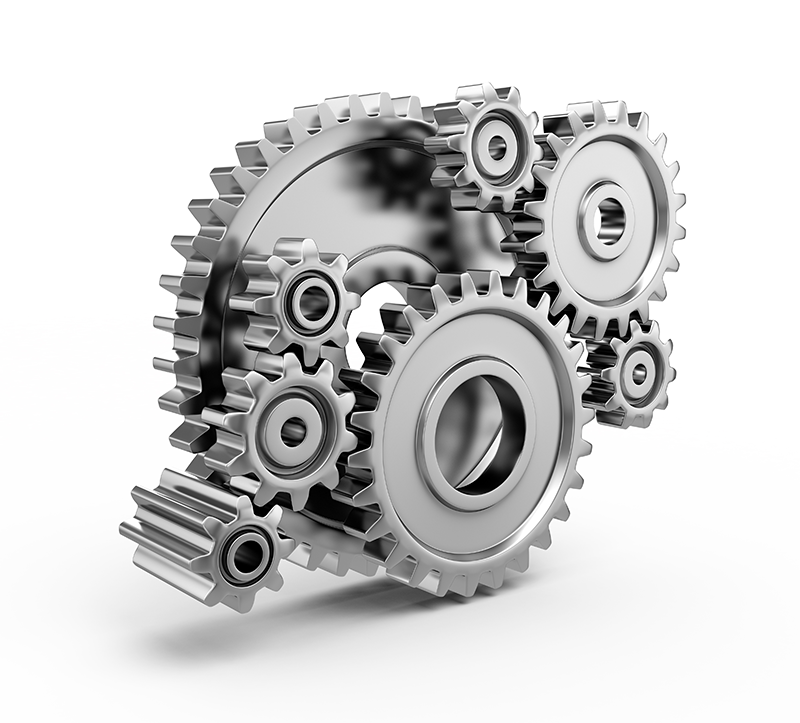
\includegraphics[width=8cm]{Src/Images/image.png}
	\caption{caption}
    \label{label}
\end{figure}

\begin{wrapfigure}{r}{8cm}
  \raggedleft
  \vspace{-2em}
  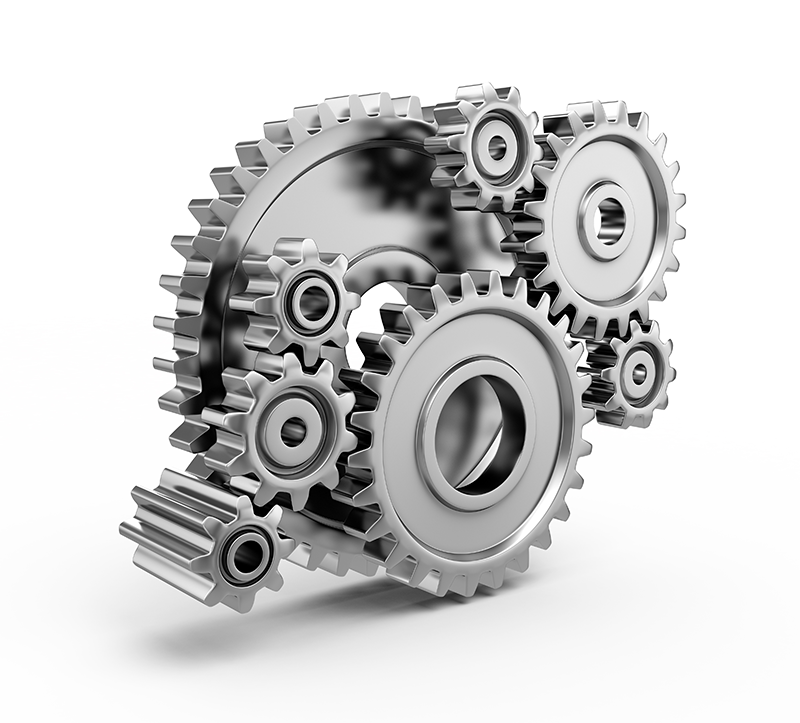
\includegraphics[width=4.5cm]{Src/Images/image.png}
  \vspace{-3em}
\end{wrapfigure}
Lorem ipsum \\ Lorem ipsum \\ Lorem ipsum \\ Lorem ipsum \\ Lorem ipsum \\ Lorem ipsum

\section{Minipages}
\noindent
\begin{minipage}[c]{0.4\linewidth}
	\centering
	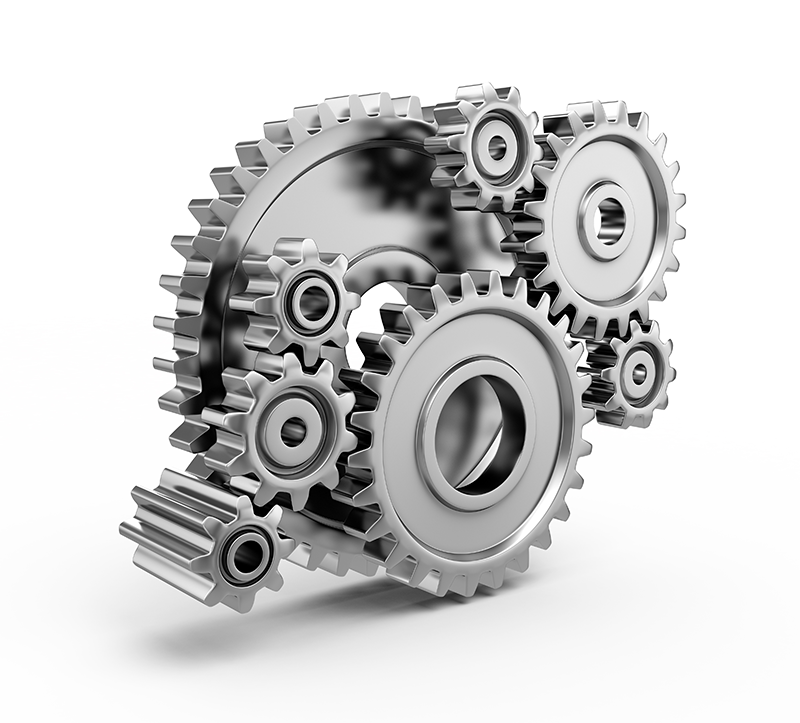
\includegraphics[width=0.9\linewidth]{Src/Images/image.png}
	\captionof{figure}{Caption}	
\end{minipage} \hfill
\begin{minipage}[c]{.5\linewidth}
	\centering
	LoremIpsum
\end{minipage} 

\begin{figure}[!ht]
\begin{minipage}[b]{.3\linewidth}
\centering
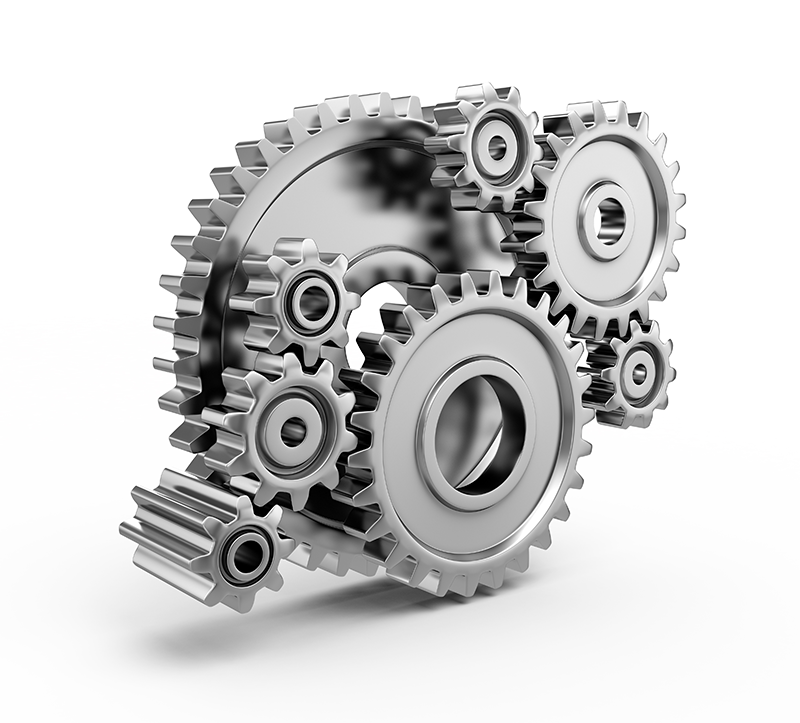
\includegraphics[width=0.9\linewidth]{Src/Images/image.png}
\subcaption{image1}
\end{minipage}%
\begin{minipage}[b]{.3\linewidth}
\centering
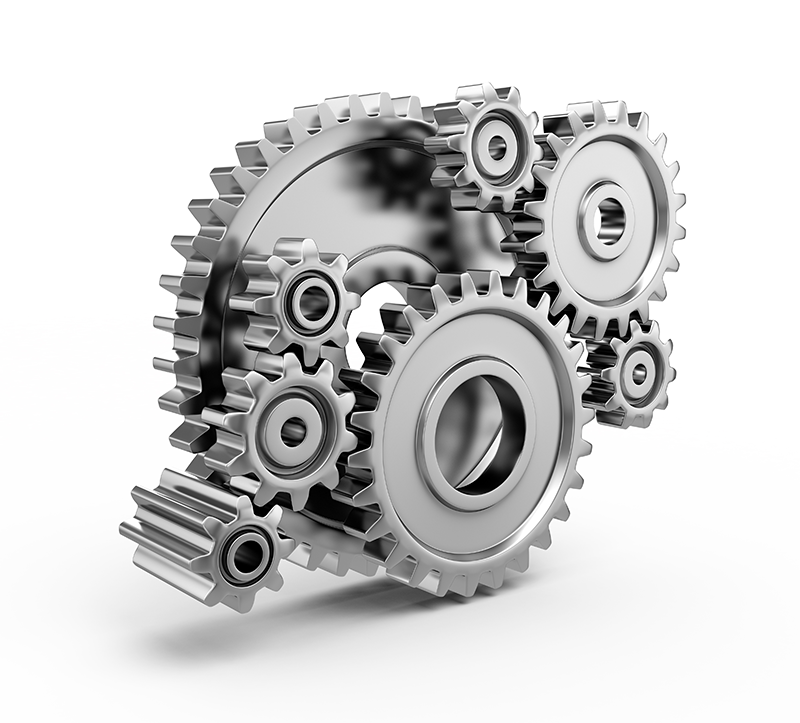
\includegraphics[width=0.9\linewidth]{Src/Images/image.png}
\subcaption{image2}
\end{minipage}
\begin{minipage}[b]{.3\linewidth}
\centering
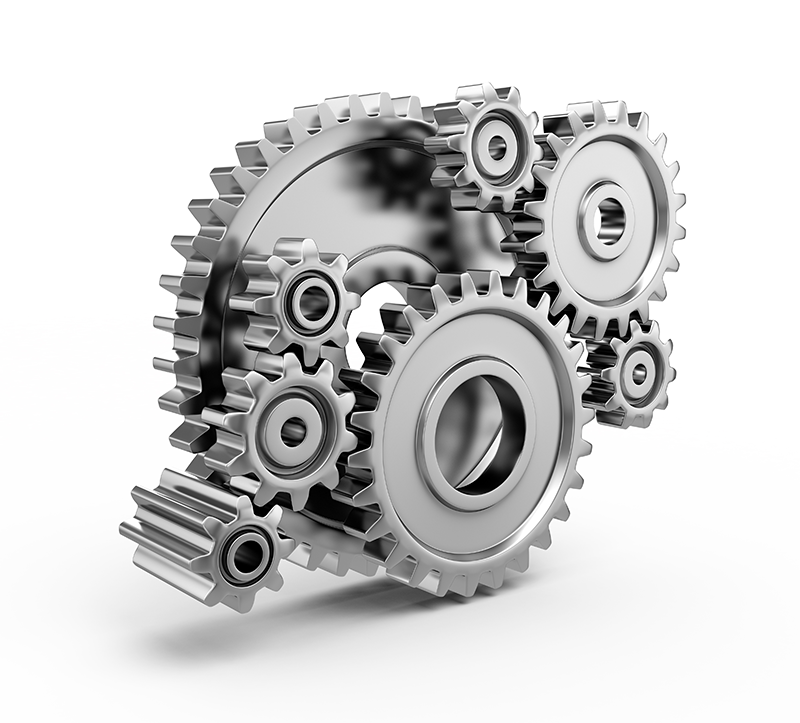
\includegraphics[width=0.9\linewidth]{Src/Images/image.png}
\subcaption{image3}
\end{minipage}
\caption{Caption}
\end{figure}


\section{Tableaux}
\begin{center}
\noindent\begin{tabular}{ >{\centering\arraybackslash} m{3cm} l l l }\toprule
A & B & C & D \\ \midrule
1 & 2 & 3 & 4 \\
1 & 2 & 3 & 4 \\ \bottomrule
\end{tabular}

\noindent\begin{tabular}{ | c | c | l | l |} \hline
A & B & C & D \\ \hline
1 & 2 & 3 & 4 \\ \hline
1 & 2 & 3 & 4 \\ \hline
\end{tabular}
\end{center}

$\left\{ \begin{array}{l}
A \\
B
\end{array} \right.$

\section{Figures de changement de base}
\vspace{-1em}
\begin{center}
\setCouleursParametrage{black}{UPSTIcustomColor1}
\parametrageAngulaire{\alpha}{\vx1}{\vy1}{\vz1}{\vx2}{\vy2}[\vz2]\qquad
\setCouleursParametrage{UPSTIcustomColor1}{UPSTIcustomColor4}
\parametrageAngulaire{\theta}{\vx1}{\vy1}{\vz1}{\vx3}{\vy3}[\vz3]

\setFigurePlaneMultipleBase0[black]{}{\vx0}{\vy0}{\vz0}
\setFigurePlaneMultipleBase1[UPSTIcustomColor1]{\alpha}{\vx{g}}{\vy{g}}{\vz{g}}
\setFigurePlaneMultipleBase2[UPSTIcustomColor3]{\beta}{\vx{g'}}{\vy{g'}}{\vz{g'}}
\setFigurePlaneMultipleBase3[UPSTIcustomColor4]{\varphi}{\vx3}{\vy3}{\vz3}
\figurePlaneMultiple[4]
\end{center}


\pagebreak
\section{Lois de vitesse}
\begin{figure}[ht]
    \centering
\begin{tikzpicture}[scale=0.3]
\draw[very thick, ->] (0,0) -- (30,0) node[right]{$t$};
\draw[very thick, ->] (0,0) -- (0,11) node[above]{\norme{\vVitesse{G}{6}{0}}};
\draw[thin, gray!60, dashed] (6,0) -- (6,9);
\draw[thin, gray!60, dashed] (20,0) -- (20,9);
\draw[thin, gray!60, dashed] (0,9) -- (6,9);
\draw(6, 0.5) -- (6, -0.5) node[below]{$T_a$};
\draw(20, 0.5) -- (20, -0.5);
\draw(20, -0.5) node[below]{$T+T_a$};
\draw(26, 0.5) -- (26, -0.5);
\draw(26, -0.5) node[below]{$T+2T_a$};
\draw(0.5, 9) -- (-0.5, 9) node[left]{$V$};
\draw[UPSTIcustomColor1,thick] [domain=0:6] plot (\x,{\x*1.5});
\draw[UPSTIcustomColor1,thick] [domain=6:20] plot (\x,{9});
\draw[UPSTIcustomColor1,thick] [domain=20:26] plot (\x,{\x*-1.5+39});
\end{tikzpicture}
	\caption{Cycle en trapèze de la loi de commande de l'actionneur}
	\label{trapeze}
\end{figure}

\begin{figure}[ht]
    \centering
\begin{tikzpicture}[scale=0.3]
\draw[very thick, ->] (0,0) -- (30,0) node[right]{$t$};
\draw[very thick, ->] (0,0) -- (0,8.5) node[above]{$V_{DDS}(t)$};
\draw[thin, gray!60, dashed] (0,6.5) -- (26,6.5);
\draw(13, 0.5) -- (13, -0.5) node[below]{$T$};
\draw(26, 0.5) -- (26, -0.5) node[below]{$2T$};
\draw(-0.5, -0.3) node[below]{0};
\draw(0.5, 6.5) -- (-0.5, 6.5) node[left]{$V_{ref}$};
\draw[UPSTIcustomColor1,thick] [domain=0:13] plot (\x,{\x*0.5});
\draw[UPSTIcustomColor1,thick] (13,0) -- (13,6.5);
\draw[UPSTIcustomColor1,thick] [domain=13:26] plot (\x,{\x*0.5-6.5});
\draw[UPSTIcustomColor1,thick] (26,0) -- (26,6.5);
\end{tikzpicture}
	\caption{Cycle en trapèze de la loi de commande de l'actionneur}
	\label{fgsdfgdsfg}
\end{figure}

\section{Graphes des liaisons}
\UPSTItitreStd{Exemple 1}

\begin{grapheLiaisons}[scale=0.55, every node/.style={scale=0.55}]
\glBati{1,0.5}{P0}{0} % Il faut ajuster ce scale en fonction du scale global du dessin
\glPiece{2.5,3}{P1}{1}
\glPiece{5,5}{P2}{2}
\glPiece{8,6}{P3}{3}
\glPiece{11,6}{P4}{4}
\glPiece{14,5}{P5}{5}
\glLiaison[bend left=10]{P0}{P1}[\liaison{0}{1}][above=0.5em,left]
\glLiaison[bend left=8]{P1}{P2}[\liaison{1}{2}][above=0.8em,left]
\glLiaison[bend left=5]{P2}{P3}[\liaison{2}{3}][left=0.5em, above]
\glLiaison[bend left=8]{P3}{P4}[\liaison{3}{4}]
\glLiaison[bend left=5]{P4}{P5}[\liaison{4}{5}][right=0.5em, above]
\end{grapheLiaisons}

\pagebreak
\UPSTItitreStd[1]{Exemple 2}

\begin{grapheLiaisons}[scale=0.3]
\glBati{0,0}{S0}{0}[1/0.3]
\glPiece{5,5}{S1}{1}
\glPiece{0,10}{S2}{2}
\glPiece{-5,5}{S3}{3}
\glLiaison[bend right=20]{S0}{S1}[Piv.\\ axe \axe{B}{\vx{}}][right]
\glLiaison[bend right=20]{S1}{S2}[Piv. Gl.\\ axe \axe{E}{\vx{}}][right]
\glLiaison[bend right=20]{S2}{S3}[Piv. Gl.\\ axe \axe{C}{\vz{}}][left]
\glLiaison[bend right=20]{S3}{S0}[Piv.\\ axe \axe{A}{\vz{}}][left]
\end{grapheLiaisons}

\UPSTItitreStd[1]{Exemple 3}

\begin{grapheLiaisons}[scale=0.4]
\glBati[-30]{0,0}{P0}{0}[1/0.4]
\glPiece{5,0}{P1}{1}
\glPiece{6.5,4.7}{P2}{2}
\glPiece{2.5,7.7}{P3}{3}
\glPiece{-1.5,4.7}{P4}{4}
\glLiaison[bend left=20, align=center, scale=0.8]{P0}{P4}[Sphérique \\ centre $A$][left]
\glLiaison[bend left=20, align=center]{P4}{P3}[Sphérique \\ centre $B$][above=0.5em, left]
\glLiaison[bend left=20, align=center]{P3}{P2}[Engrenage][above=0.5em, right]
\glLiaison[bend left=20, align=center]{P2}{P1}[Glissière \\ dir. $x_1$][right]
\glLiaison[bend left=20, align=center]{P1}{P0}[Pivot \\ axe \axe{O}{\vz{}}][below]

\draw[thick,<-,>=latex,UPSTIcustomColor1](P1)to[bend right]++(2,-1.5)node[right]{\tAM{\text{air}}{\text{pales}}};

\end{grapheLiaisons}


\UPSTItitreStd[1]{Exemple 4}

\begin{grapheLiaisons}[scale=0.5]
\glBati[-90]{0,0}{P0}{0}[1/0.5]
\glPiece{10,0}{P1}{1}
\glPiece{5,3}{V1}{$v_1$}
\glPiece{5,0}{V2}{$v_2$}
\glPiece{5,-3}{V3}{$v_3$}
\glLiaison[bend left=20]{P0}{V1}[\liaison{0}{v_1}][above=0.2em]
\glLiaison{P0}{V2}[\liaison{0}{v_2}][above]
\glLiaison[bend right=20]{P0}{V3}[\liaison{0}{v_3}][below=0.2em]
\glLiaison[bend left=20]{V1}{P1}[\liaison{1}{v_1}][above=0.2em]
\glLiaison{V2}{P1}[\liaison{1}{v_2}][above]
\glLiaison[bend right=20]{V3}{P1}[\liaison{1}{v_3}][below=0.2em]
\end{grapheLiaisons}

\UPSTItitreStd[1]{Exemple 5}

\begin{grapheLiaisons}[scale=0.5]
\glPiece{0,0}{S1}{$S_1$}
\glPiece{15,0}{S2}{$S_2$}
\glLiaison[bend left=20]{S1}{S2}[Liaison équi. 1]
\glLiaison[bend right=20]{S1}{S2}[Liaison équi. 2][below]
\end{grapheLiaisons}

\UPSTItitreStd[1]{Exemple 6}

\begin{grapheLiaisons}[scale=0.5]
\glPiece{0,0}{S1}{$S_1$}
\glPiece{15,0}{S2}{$S_2$}
\glLiaison{S1}{S2}[Liaison équi. globale]
\end{grapheLiaisons}

\UPSTItitreStd[1]{Exemple 7}

\begin{grapheLiaisons}[scale=0.55]
\glBati[-45]{1,0.5}{P1}{1}[1/0.55]
\glPiece{4,3.5}{P2}{2}
\glPiece{7,0.5}{P3}{3}
\glLiaison[bend left]{P1}{P2}[Pivot\\ axe \axe{O_1}{\vz1}][above=0.8em,left]
\glLiaison[bend left]{P2}{P3}[Lin. Rect.\\ dir. \vz1][above=0.8em,right]
\glLiaison[bend left=10]{P3}{P1}[Piv. Gl.\\ axe \axe{D}{\vy1}]
\end{grapheLiaisons}

\UPSTItitreStd[1]{Exemple 8}

\begin{grapheLiaisons}[scale=0.45]
\glBati{1,0.5}{P0}{0}[1/0.45]
\glPiece{4,5}{P1}{1}
\glPiece{10,2}{P2}{2}
\glLiaison[bend left]{P0}{P1}[Piv. Gl.\\ axe \axe{B}{\vx{}}][above=0.8em,left]
\glLiaison[bend right]{P0}{P1}[Piv. Gl.\\ axe \axe{C}{\vx{}}][right=-0.5em]
\glLiaison[bend left]{P1}{P2}[Gl. Hélic.\\ axe \axe{A}{\vx{}}][above=0.8em,right]
\glLiaison[bend left]{P2}{P0}[Piv. axe \axe{A}{\vx{}}][below]
\end{grapheLiaisons}

\UPSTItitreStd[1]{Exemple 9}

\begin{grapheLiaisons}[scale=0.55]
\glBati{0,0}{P0}{0}[1/0.55]
\glPiece{-5,5}{P1}{1}
\glPiece{0,8}{P2}{2}
\glPiece{5,5}{P3}{3}
\glLiaison[bend left]{P0}{P1}[\glDeuxL{Piv. Gl.}{axe \axe{A}{\vz{}}}][left]
\glLiaison[bend right=10]{P0}{P1}[\glDeuxL{Piv. Gl.}{axe \axe{B}{\vz{}}}][below=1em, right]
\glLiaison[bend right]{P0}{P3}[Pct][right]
\glLiaison[bend left]{P1}{P2}[\glDeuxL{Piv.}{axe \axe{K}{\vx{}}}][left]
\glLiaison[bend left=10]{P1}{P3}[\glDeuxL{Rot.}{centre $C'$}][above]
\glLiaison[bend right=10]{P1}{P3}[LA \axe{C}{\vy{}}][below]
\glLiaison[bend left]{P2}{P3}[Pct][right]
\end{grapheLiaisons}

\UPSTItitreStd[1]{Exemple 10}

\begin{grapheLiaisons}[scale=0.4]
\glBati{0,0}{P1}{1}[1/0.4]
\glPiece{-5,5}{P24}{24}
\glPiece{0,10}{P4}{4}
\glPiece{5,5}{P7}{7}
\glPiece{15,0}{P10}{10}
\glPiece{15,10}{P11}{11}
\glLiaison[bend left]{P1}{P24}[\glDeuxL{Piv.}{axe \axe{A}{\vx{}}}][left]
\glLiaison[bend left]{P1}{P4}[\glDeuxL{Piv.}{axe \axe{B}{\vx{}}}][right=-1em]
\glLiaison[bend right]{P1}{P7}[\glDeuxL{Piv. Gl.}{axe \axe{C}{\vx{}}}][below]
\glLiaison[bend right]{P4}{P24}[\glDeuxL{RSG}{normale \axe{E}{\vy{}}}][left]
\glLiaison[bend left]{P4}{P7}[\glDeuxL{Gl. Hél.}{axe \axe{B}{\vx{}}}][above]
\glLiaison[bend left=10]{P7}{P10}[\glDeuxL{Piv.}{axe \axe{C}{\vx{}}}][below]
\glLiaison[bend right=10]{P7}{P11}[\glDeuxL{Piv.}{axe \axe{D}{\vx{}}}][above]
\glLiaison[bend right]{P10}{P11}[\glDeuxL{RSG}{normale \axe{F}{\vy{}}}][right]
\end{grapheLiaisons}


\section{Schémas blocs}
\UPSTItitreStd{Exemple 1}

\begin{tikzpicture}
\sbEntree{E}
\sbComp[5]{comp}{E}
	\sbRelier[$E(p)$]{E}{comp}
\sbChaine[5]{comp}{B/$H(p)$}
\sbDecaleNoeudy[5]{B}{DebutRetour}
\node[above of=comp-B,node distance=0.5em]{$e(p)$};
\sbChaineRetour[0]{DebutRetour}{K/$K(p)$}
\sbRelierxy[$M(p)$]{K}{comp}
\sbSortie[5]{S}{B}
\sbRelier{B}{S}
\sbRelieryx{B-S}{K}
\node[above of=S,node distance=0.82em]{$V(p)$};
\draw [gray, dashed] (1.3,-2.8) rectangle (6.7,0.9);
\end{tikzpicture}

\UPSTItitreStd[1]{Exemple 2}

\begin{tikzpicture}
\sbEntree{E}
\sbBloc[4]{G}{$G(p)$}{E}
\sbRelier[$E(p)$]{E}{G}
\sbSortie[4]{S}{G}
\sbRelier[$S(p)$]{G}{S}
\end{tikzpicture}

\UPSTItitreStd[1]{Exemple 3}

\begin{tikzpicture}
\sbEntree{E1}
\sbStyleBloc{align=center}
\sbBloc[12]{Bloc1}{Variateur de vitesse \\ pour machine \\ asynchrone \\ triphasée}{E1}
\sbStyleLien{align=center}
\sbRelier[Énergie électrique \\ à valeur efficace et \\ fréquence fixes]{E1}{Bloc1}
\sbSortie[12]{S1}{Bloc1}
\sbRelier[Énergie électrique \\ à valeur efficace et \\ fréquence variables]{Bloc1}{S1}
\end{tikzpicture} 

\UPSTItitreStd[1]{Exemple 4}

\begin{tikzpicture}
\sbEntree{E1}
\sbBloc{B0}{Énergie électrique}{E1}
\sbBlocL{B1}{Moteur}{B0}
\sbBlocL{B2}{Réducteur}{B1}
\sbBlocL{B3}{Biellette}{B2}
\sbBlocL{B4}{Lice}{B3}
\end{tikzpicture} 

\UPSTItitreStd[1]{Exemple 5}

\begin{tikzpicture}
\sbEntree{E}
\sbCompSum{comp}{E}{}{}{}{}
\sbRelier[$U(p)$]{E}{comp}
\sbBlocL{a}{$\phantom{123456789}$}{comp}
\sbBloc[3]{b}{$\phantom{123456789}$}{a}
\sbRelier[$I(p)$]{a}{b}
\sbSortie[3]{S}{b}
\sbRelier[$C_r(p)$]{b}{S}
\sbDecaleNoeudy[-4]{adroite}{dd}
\sbBlocr[0]{d}{$\phantom{123456789}$}{dd}
\sbRelierxy{d}{comp}
\sbDecaleNoeudx[3]{dd}{ddd}
\draw[->,>=latex'](ddd) -- (d) node[midway, above] {$\Omega(p)$};
\end{tikzpicture}

\UPSTItitreStd[1]{Exemple 6}

\begin{tikzpicture}
\sbEntree{E}
\sbComp{comp}{E}
\sbRelier[$V(p)$]{E}{comp}
\sbBloc[3]{a}{$K_i$}{comp}
\sbRelier[$\varepsilon_i(p)$]{comp}{a}
\sbBloc[3]{b}{Moteur}{a}
\sbRelier[$U(p)$]{a}{b}
\sbSortie[3]{S}{b}
\sbRelier[$C_r(p)$]{b}{S}
\sbDecaleNoeudy[4]{adroite}{cc}
\sbBlocr[0]{c}{$R_m$}{cc}
\draw[->,>=latex'] (b) |- (c) node[pos=.5,above left] {$I(p)$};
\draw[->,>=latex'] (c) -| (comp) node[pos=.5,above right] {$V_i(p)$};
\draw[->,>=latex'] ($(b)+(0,1)$) node [above] {$\Omega(p)$} -- (b);
\end{tikzpicture}

\UPSTItitreStd[1]{Exemple 7}

\noindent\resizebox{\linewidth}{!}{
\begin{tikzpicture}
\sbEntree{E}
\sbBloc[3]{z}{Adaptateur}{E}
\sbRelier[$C^*_r(p)$]{E}{z}
\sbComp[6]{comp}{z}
\sbRelier{z}{comp}
\sbBloc[3]{a}{Correcteur}{comp}
\sbRelier[$\varepsilon_c(p)$]{comp}{a}
\sbBloc[3]{b}{Moteur + boucle de courant}{a}
\sbRelier[$V(p)$]{a}{b}
\sbSortie[4]{S}{b}
\sbRelier{b}{S}
\sbDecaleNoeudy[4]{b}{cc}
\sbBlocr[0]{c}{Capteur + conditionneur}{cc}
\draw[->,>=latex'] ($(b-S.south)+(.4,0)$) coordinate (d) node[above right] {$C_r(p)$} |- (c) ;
\draw[->,>=latex'] (c) -| (comp) node[pos=.5,above right] {$C(p)$};
\sbDecaleNoeudy[-4]{b-S}{dd}
\sbBlocr{e}{Charge}{dd}
\sbRelieryx{b-S}{e}
\draw[->,>=latex'] (e)  -| (b) node[pos=.5,below left] {$\Omega(p)$};
\end{tikzpicture}
}

\UPSTItitreStd[1]{Exemple 8}

\begin{tikzpicture}
\sbEntree{E}
\sbComp{comp}{E}
\sbRelier[$C_r^*(p)$]{E}{comp}
\sbBlocL{A}{$\textrm{FTCD}(p)$}{comp}
\sbSortie[3]{S}{A}
\sbRelier[$C_r(p)$]{A}{S}
\sbDecaleNoeudy[4]{Adroite}{bb}
\sbBlocr[0]{B}{$\textrm{FTCR}(p)$}{bb}
\sbRelieryx{A-S}{B}
\sbRelierxy{B}{comp}
\end{tikzpicture}

\UPSTItitreStd[1]{Exemple 9}

\begin{tikzpicture}
\sbEntree{E}
\sbComp[6]{comp}{E}
\sbStyleBloc{align=center}
\sbStyleLien{align=center}
\sbRelier[Tension de \\ consigne]{E}{comp}
\sbBloc{CC}{Carte de \\ commande}{comp}
\sbRelier{comp}{CC}
\sbBloc[4]{Mot}{Moteur}{CC}
\sbRelier[$U_{mot}$]{CC}{Mot}
\sbBloc[4]{Red}{Réducteur-Chaîne \\ Chariot-corde}{Mot}
\sbRelier[$C_{mot}$]{Mot}{Red}
\sbSortie[5]{S}{Red}
\sbRelier[Tension]{Red}{S}
\sbDecaleNoeudy[5]{Red}{DebutRetour}
\sbChaineRetour[2]{DebutRetour}{Res/Ressort \\ K,Cap/Capteur \\ position}
\sbRelieryx{Red-S}{Res}
\sbRelierxy[Tension \\ mesurée]{Cap}{comp}
%\draw[dotted] (6.5,-1) rectangle (11.5,-3.5);
\draw[dotted] (6.5,-3.3) -- (6.5,-1) -- (11.5,-1) -- (11.5,-3.3) -- (6.5,-3.3) node[midway,above] {Capteur d'effort};
\end{tikzpicture}

\pagebreak
\UPSTItitreStd[1]{Exemple 10}

\begin{tikzpicture}
\sbEntree{Ent}
\sbComp[4]{Comp}{Ent}
\sbStyleBloc{align=center}
\sbStyleLien{align=center}
\sbRelier[$U$]{Ent}{Comp}
\sbBloc{A}{Correcteur}{Comp}
\sbRelier{Comp}{A}
\sbBloc{B}{Moteur}{A}
\sbRelier{A}{B}
\sbBloc{C}{Réducteur}{B}
\sbRelier[$\Omega_M$]{B}{C}
\sbBloc{D}{Poulie \\ courroie}{C}
\sbRelier[$\Omega_R$]{C}{D}
\sbBloc{E}{Tapis + \\ chariot}{D}
\sbRelier[$V_C$]{D}{E}
\sbSortie[3]{Sor}{E}
\sbRelier[$V_T$]{E}{Sor}
\sbDecaleNoeudy[5]{E}{DebutRetour}
\sbChaineRetour[8]{DebutRetour}{RA/Capteur}
\sbRelieryx{E-Sor}{RA}
\sbRelierxy{RA}{Comp}
\end{tikzpicture}

\UPSTItitreStd[1]{Exemple 11}

\begin{tikzpicture}
\sbEntree{Ent}
\sbComp[4]{Comp}{Ent}
\sbStyleBloc{align=center}
\sbStyleLien{align=center}
\sbRelier[$Cde$]{Ent}{Comp}
\sbBloc{A}{Correcteur}{Comp}
\sbRelier[$\varepsilon$]{Comp}{A}
\sbBloc{B}{Hacheur}{A}
\sbRelier{A}{B}
\sbBloc[3]{C}{Moteur}{B}
\sbRelier[$U(p)$]{B}{C}
\sbBloc[3]{D}{?}{C}
\sbRelier[$\Omega (p)$]{C}{D}
\sbDecaleNoeudy[5]{D}{DebutRetour}
\sbChaineRetour[8]{DebutRetour}{RA/Codeur}
\sbRelieryx{D-E}{RA}
\sbRelierxy[Image de la position]{RA}{Comp}
\sbBloc[3]{E}{?}{D}
\sbRelier[$\theta (p)$]{D}{E}
\sbSortie[3]{Sor}{E}
\sbRelier[$\theta_r (p)$]{E}{Sor}
\end{tikzpicture}

\UPSTItitreStd[1]{Exemple 12}

\noindent\resizebox{\linewidth}{!}{
\begin{tikzpicture}
\sbStyleBloc{align=center}
\sbStyleLien{align=center}
\sbEntree{Ent}
\sbBloc[4]{A}{$H1$}{Ent}
\sbRelier[$\theta_{\text{consigne}}$]{Ent}{A}
\sbComp{Comp}{A}
\sbRelier{A}{Comp}
\sbBloc[1]{B}{$H2$}{Comp}
\sbRelier{Comp}{B}
\sbBloc[1]{C}{$H3$}{B}
\sbRelier{B}{C}
\sbBloc[1]{D}{$H4$}{C}
\node [above=1.5em of C] (CC) {$24\siUV$};
\draw[-latex] (CC) -- (C.north);
\sbRelier{C}{D}
\sbBloc[1]{E}{$H5$}{D}
\sbRelier{D}{E}
\sbBloc[1]{F}{$H6$}{E}
\sbRelier{E}{F}
\sbBloc[1]{G}{$H7$}{F}
\sbRelier{F}{G}
\sbBloc[3]{H}{$H8$}{G}
\sbRelier[$\Omega_{\text{bras}}$]{G}{H}
\sbSortie[3]{Sor}{H}
\sbRelier[$\theta_{\text{bras}}$]{H}{Sor}
\sbDecaleNoeudy[5]{H}{DebutRetour}
\sbChaineRetour[4]{DebutRetour}{RA/$H9$,RB/$H10$}
\sbRelieryx{H-Sor}{RA}
\sbRelierxy{RB}{Comp}
\node[below = 1cm of Ent-A] (txtEnt-A) {étiquette};
\end{tikzpicture}
}

\UPSTItitreStd[1]{Exemple 13}

\noindent\resizebox{\linewidth}{!}{
\begin{tikzpicture}
\sbEntree{Ent}
\sbBloc[3]{IHM}{IHM}{Ent}
\sbRelier[$V_c(t)$]{Ent}{IHM}
\sbComp[5]{Comp}{IHM}
\sbRelier[$u_{\Omega_c}(t)$]{IHM}{Comp}
\sbBloc{A}{Calculateur}{Comp}
\sbRelier[$\varepsilon(t)$]{Comp}{A}
\sbBloc[3]{B}{Hacheur}{A}
\sbRelier[$u_{com}(t)$]{A}{B}
\sbBloc[3]{C}{Moteur}{B}
\sbRelier[$u_m(t)$]{B}{C}
\sbBloc[3]{D}{Réducteur}{C}
\sbRelier[$\Omega_m(t)$]{C}{D}
\sbDecaleNoeudy[5]{D}{DebutRetour}
\sbChaineRetour[8]{DebutRetour}{RA/Capteur de $\omega$}
\sbRelierxy[$u_{\Omega}(t)$]{RA}{Comp}
\sbBloc[3]{E}{Tapis}{D}
\sbRelier[$\Omega_R(t)$]{D}{E}
\sbSortie[2]{Sor}{E}
\sbRelier[$V(t)$]{E}{Sor}
\sbRelieryx{D-E}{RA}
\end{tikzpicture}
}

\UPSTItitreStd[1]{Exemple 14}

\noindent\resizebox{\linewidth}{!}{
\begin{tikzpicture}
\sbEntree{E}
\sbComp{comp1}{E}
\sbRelier{E}{comp1}
\draw (E) node[above]{$U(p)$};
\sbBlocL{aa}{$\dfrac{\eta K_t}{R+Lp}$}{comp1}
\sbBloc[4]{a}{$\dfrac{1}{R_r}$}{aa}
\sbRelier[$C_{S-R}(p)$]{aa}{a}
\sbComp{comp2}{a}
\sbRelier{a}{comp2}
\sbBloc[4]{b}{$6$}{comp2}
\sbRelier[$F_{R-S}(p)$]{comp2}{b}
\sbSumh{comp3}{b}
\sbRelier{b}{comp3}
\sbDecaleNoeudy[-4]{comp3}{E2}
\sbRelier{E2}{comp3}
\draw (E2) node[below left]{$F_{V-S}(p)$};
\sbBlocL{c}{$\dfrac{1}{M_s p^2}$}{comp3}
\sbSortie[5]{S}{c}
\sbRelier{c}{S}
\draw (S) node[above]{$X_s(p)$};
\sbDecaleNoeudy[4]{comp3}{dd}
\sbBlocr[0]{d}{$\left(M_r+\dfrac{I_r}{R_r^2}\right) p^2$}{dd}
\sbRelieryx{c-S}{d}
\sbRelierxy{d}{comp2}
\sbDecaleNoeudy[8]{comp3}{ddd}
\sbBlocr[0]{e}{$\dfrac{\eta K_e}{R_r}p$}{ddd}
\sbSortie[4]{ss}{c}
\sbRelieryx{ss}{e}
\sbRelierxy{e}{comp1}
\end{tikzpicture}
}

\UPSTItitreStd[1]{Exemple 15}

\begin{tikzpicture}
\sbEntree{E}
\draw (E) node[above]{$U(p)$};
\sbComp{comp2}{E}
\sbRelier{E}{comp2}
\sbBloc{a}{$A$}{comp2}
\sbRelier{comp2}{a}
\sbSumh{comp3}{a}
\sbRelier{a}{comp3}
\sbDecaleNoeudy[-4]{comp3}{E2}
\sbRelier{E2}{comp3}
\draw (E2) node[below left]{$F_{V-S}(p)$};
\sbBlocL{c}{$B$}{comp3}
\sbSortie{S}{c}
\sbRelier{c}{S}
\draw (S) node[above]{$X_s(p)$};
\sbDecaleNoeudy[4]{comp3}{dd}
\sbBlocr[0]{d}{$D$}{dd}
\sbRelieryx{c-S}{d}
\sbRelierxy{d}{comp2}
\end{tikzpicture}

\UPSTItitreStd[1]{Exemple 16}

\begin{tikzpicture}
\sbEntree{E}
\draw (E) node[above]{$X_c(p)$};
\sbComp{comp}{E}
\sbRelier{E}{comp}
\sbBloc{corr}{$C(p)$}{comp}
\sbRelier{comp}{corr}
\sbComp{comp2}{corr}
\sbRelier{corr}{comp2}
\sbBloc{a}{$A$}{comp2}
\sbRelier{comp2}{a}
\sbSumh{comp3}{a}
\sbRelier{a}{comp3}
\sbDecaleNoeudy[-4]{comp3}{E2}
\sbRelier{E2}{comp3}
\draw (E2) node[below left]{$F_{V-S}(p)$};
\sbBlocL{c}{$B$}{comp3}
\sbSortie{S}{c}
\sbRelier{c}{S}
\draw (S) node[above]{$X_s(p)$};
\sbDecaleNoeudy[4]{comp3}{dd}
\sbBlocr[0]{d}{$D$}{dd}
\sbRelieryx{c-S}{d}
\sbRelierxy{d}{comp2}
\coordinate (toto) at ($(c-S.south)+(1mm,0)$);
\sbRenvoi[6]{toto}{comp}{}
\end{tikzpicture}

\UPSTItitreStd[1]{Exemple 17}

\begin{tikzpicture}
\sbEntree{E}
\draw (E) node[above]{$C_{S-R}(p)$};
\sbBlocL[4]{a}{$\dfrac{1}{R_r}$}{E}
\sbComp{comp2}{a}
\sbRelier{a}{comp2}
\sbBloc[4]{b}{$6$}{comp2}
\sbRelier[$F_{R-S}(p)$]{comp2}{b}
\sbSumh{comp3}{b}
\sbRelier{b}{comp3}
\sbDecaleNoeudy[-4]{comp3}{E2}
\sbRelier{E2}{comp3}
\draw (E2) node[below left]{$F_{V-S}(p)$};
\sbBlocL{c}{$\dfrac{1}{M_s p^2}$}{comp3}
\sbSortie{S}{c}
\sbRelier{c}{S}
\draw (S) node[above]{$X_s(p)$};
\sbDecaleNoeudy[4]{comp3}{dd}
\sbBlocr[0]{d}{$\left(M_r+\dfrac{I_r}{R_r^2}\right) p^2$}{dd}
\sbRelieryx{c-S}{d}
\sbRelierxy{d}{comp2}
\end{tikzpicture}

\UPSTItitreStd[1]{Exemple 18}

\noindent\resizebox{\linewidth}{!}{
\begin{tikzpicture}
\sbEntree{E}
\sbComp{comp1}{E}
\sbRelier{E}{comp1}
\draw (E) node[above]{$U(p)$};
\sbBlocL{aa}{}{comp1}
\sbBloc[4]{a}{$\dfrac{1}{R_r}$}{aa}
\sbRelier[$C_{S-R}(p)$]{aa}{a}
\sbComp{comp2}{a}
\sbRelier{a}{comp2}
\sbBloc[4]{b}{$6$}{comp2}
\sbRelier[$F_{R-S}(p)$]{comp2}{b}
\sbSumh{comp3}{b}
\sbRelier{b}{comp3}
\sbDecaleNoeudy[-4]{comp3}{E2}
\sbRelier{E2}{comp3}
\draw (E2) node[below left]{$F_{V-S}(p)$};
\sbBlocL{c}{$\dfrac{1}{M_s p^2}$}{comp3}
\sbSortie[5]{S}{c}
\sbRelier{c}{S}
\draw (S) node[above]{$X_s(p)$};
\sbDecaleNoeudy[4]{comp3}{dd}
\sbBlocr[0]{d}{$\left(M_r+\dfrac{I_r}{R_r^2}\right) p^2$}{dd}
\sbRelieryx{c-S}{d}
\sbRelierxy{d}{comp2}
\sbDecaleNoeudy[8]{comp3}{ddd}
\sbBlocr[0]{e}{}{ddd}
%\sbDecaleNoeudx[1]{c-S}{ss}
\sbSortie[4]{ss}{c}
\sbRelieryx{ss}{e}
\sbRelierxy{e}{comp1}
\end{tikzpicture}
}

\UPSTItitreStd[1]{Exemple 19}

\noindent\resizebox{\linewidth}{!}{
\begin{tikzpicture}
\sbEntree{E}
\sbComp{comp}{E}
\sbRelier[$Q(p)$]{E}{comp}
\sbBloc[1]{a}{$xxx$}{comp}
\sbRelier{comp}{a}
\sbBloc[1]{ab}{$\dfrac{1}{p}$}{a}
\sbRelier{a}{ab}
\sbBloc[3]{ac}{$yyy$}{ab}
\sbRelier[$\Sigma (p)$]{ab}{ac}
\sbComph[5]{b}{ac}
\sbRelier[$F(p)$]{ac}{b}
\sbBloc[1]{ba}{$zzz$}{b}
\sbRelier{b}{ba}
\sbBloc[3]{bb}{$aaa$}{ba}
\sbRelier[$\Gamma (p)$]{ba}{bb}
\sbBloc[3]{bc}{$bbb$}{bb}
\sbRelier[$V(p)$]{bb}{bc}
\sbSortie[4]{S}{bc}
\sbRelier{bc}{S}
\node [above=0em of S] (TextS) {$Y(p)$};
\sbDecaleNoeudy[4]{b}{cc}
\sbDecaleNoeudy[5]{bb-bc}{ee}
\sbBlocr[12]{f}{$ddd$}{ee}
\sbRelieryx{bb-bc}{f}
\draw[->,>=latex'] (f)  -| (comp) node[pos=.5,below left] {$ $};
\sbDecaleNoeudy[-4]{bc-S}{dd}
\sbBlocr[8]{e}{$eee$}{dd}
\sbRelieryx{bc-S}{e}
\draw[->,>=latex'] (e)  -| (b) node[pos=.5,below left] {$ $};
\end{tikzpicture}
}

\UPSTItitreStd[1]{Exemple 20}

\noindent\resizebox{\linewidth}{!}{
\begin{tikzpicture}
\sbEntree{E}
\sbBloc[3]{g}{50}{E}
\sbRelier[$Y_c(p)$]{E}{g}
\sbComp{comp1}{g}
\sbRelier{g}{comp1}
\sbBloc[1]{a}{$C'(p)$}{comp1}
\sbRelier{comp1}{a}
\sbComp[5]{comp2}{a}
\sbRelier[$V_c(p)$]{a}{comp2}
\sbBloc[1]{ab}{$C(p)$}{comp2}
\sbRelier{comp2}{ab}
\sbBloc[3]{ac}{$A$}{ab}
\sbRelier[$U(p)$]{ab}{ac}
\sbBloc[3]{b}{$G$}{ac}
\sbRelier[$I(p)$]{ac}{b}
\sbBloc[3]{c}{$\dfrac{\delta}{1+\frac{p^2}{\beta^2}}$}{b}
\sbRelier[$Q(p)$]{b}{c}
\sbBloc[3]{cd}{$\dfrac{1}{p}$}{c}
\sbRelier[$V(p)$]{c}{cd}
\sbSortie[2]{S}{cd}
\sbRelier{cd}{S}
\draw (S) node[above]{$Y(p)$};
\sbDecaleNoeudy[4]{c}{dd}
\sbBlocr[3]{d}{$g$}{dd}
\sbBlocr[3]{de}{$1+\tau p$}{d}
\sbRelier{d}{de}
\sbRelieryx{c-cd}{d}
\sbRelierxy{de}{comp2}
\sbDecaleNoeudy[8]{cd}{ddd}
\sbBlocr[15]{e}{$h$}{ddd}
\sbSortie[1]{ss}{cd}
\sbRelieryx{ss}{e}
\sbRelierxy{e}{comp1}
\end{tikzpicture}
}

\UPSTItitreStd[1]{Exemple 21}

\begin{tikzpicture}
\sbEntree{E}
\sbBloc[3]{A}{$\dfrac{4}{3}$}{E}
\sbComp{comp}{A}
\sbRelier[$\theta_c(t)$]{E}{A}
\sbRelier{A}{comp}
\sbSortie[3]{S}{comp}
\sbRelier[$\theta_e(t)$]{comp}{S}
\sbDecaleNoeudy[4]{compdroite}{ddt}
\sbDecaleNoeudx[3]{ddt}{dd}
\sbBlocr[0]{d}{$\dfrac{1}{3}$}{dd}
\sbRelierxy{d}{comp}
\sbDecaleNoeudx[2]{dd}{ddd}
\draw[->,>=latex'](ddd) -- (d);
\node at (2.5,-1.1) {$\theta_r(t)$};
\end{tikzpicture}

\UPSTItitreStd[1]{Exemple 22}

\begin{tikzpicture}
\sbEntree{Ent}
\sbComp[4]{Comp}{Ent}
\sbStyleBloc{align=center}
\sbStyleLien{align=center}
\sbRelier[$\Delta P_{cs}$]{Ent}{Comp}
\sbBloc[3]{A}{Correcteur}{Comp}
\sbRelier[$\varepsilon (p)$]{Comp}{A}
\sbBloc[3]{B}{Soupape}{A}
\sbRelier[$\Delta x$]{A}{B}
\sbBloc[3]{C}{Turbine}{B}
\sbRelier[$\Delta q$]{B}{C}
\sbSortie[3]{Sor}{C}
\sbRelier[$\Delta P_m$]{C}{Sor}
\sbRenvoi{C-Sor}{Comp}{}
\end{tikzpicture}

\UPSTItitreStd[1]{Exemple 23}

\begin{tikzpicture}
\sbEntree{Ent}
\sbBloc[3]{IHM}{IHM}{Ent}
\sbRelier[$\theta_c(p)$]{Ent}{IHM}
\sbComp[5]{Comp}{IHM}
\sbRelier[$U_c(p)$]{IHM}{Comp}
\sbBloc{A}{$C$}{Comp}
\sbRelier[$\varepsilon(p)$]{Comp}{A}
\sbBloc[3]{B}{$H_m(p)$}{A}
\sbRelier[$U(p)$]{A}{B}
\sbBloc[3]{C}{$r$}{B}
\sbRelier[$\Omega_2(p)$]{B}{C}
\sbBloc[3]{D}{$\dfrac{1}{p}$}{C}
\sbRelier[$\Omega_4(p)$]{C}{D}
\sbDecaleNoeudy[5]{D}{DebutRetour}
\sbChaineRetour[8]{DebutRetour}{RA/$K_c$}
\sbRelierxy[$U'(p)$]{RA}{Comp}
\sbSortie[3]{Sor}{D}
\sbRelier[$\theta_p(p)$]{D}{Sor}
\sbRelieryx{D-Sor}{RA}
\end{tikzpicture}

\section{Diagrammes pédagogiques}
\begin{center}

\UPSTIdiagrammeCompetences

\UPSTIdiagrammeCompetences[0.55][1][1][1][0]

\vspace{3em}

\UPSTIdiagrammeEcarts[][1][0][1]

\end{center}


\section{Boites pour activités}
\begin{UPSTIactivite}[0]
\begin{itemize}
\item Mise en forme pour \UPSTIcode{\textbackslash begin{UPSTIactivite}[0]}
\end{itemize}
\end{UPSTIactivite} 

\begin{UPSTIactivite}[1]
\begin{itemize}
\item Mise en forme pour \UPSTIcode{\textbackslash begin{UPSTIactivite}[1]}
\end{itemize}
\end{UPSTIactivite} 

\begin{UPSTIactivite}[2]
\begin{itemize}
\item Mise en forme pour \UPSTIcode{\textbackslash begin{UPSTIactivite}[2]}
\end{itemize}
\end{UPSTIactivite} 

\begin{UPSTIactivite}[3]
\begin{itemize}
\item Mise en forme pour \UPSTIcode{\textbackslash begin{UPSTIactivite}[3]}
\end{itemize}
\end{UPSTIactivite} 

\begin{UPSTIactivite}[4]
\begin{itemize}
\item Mise en forme pour \UPSTIcode{\textbackslash begin{UPSTIactivite}[4]}
\end{itemize}
\end{UPSTIactivite} 

\begin{UPSTIactivite}[5]
\begin{itemize}
\item Mise en forme pour \UPSTIcode{\textbackslash begin{UPSTIactivite}[5]}
\end{itemize}
\end{UPSTIactivite} 

\begin{UPSTIactivite}[6]
\begin{itemize}
\item Mise en forme pour \UPSTIcode{\textbackslash begin{UPSTIactivite}[6]}
\end{itemize}
\end{UPSTIactivite} 

\begin{UPSTIactivite}[7]
\begin{itemize}
\item Mise en forme pour \UPSTIcode{\textbackslash begin{UPSTIactivite}[7]}
\end{itemize}
\end{UPSTIactivite} 

\begin{UPSTIactivite}[8]
\begin{itemize}
\item Mise en forme pour \UPSTIcode{\textbackslash begin{UPSTIactivite}[8]}
\end{itemize}
\end{UPSTIactivite} 

\begin{UPSTIactivite}[9]
\begin{itemize}
\item Mise en forme pour \UPSTIcode{\textbackslash begin{UPSTIactivite}[9]}
\end{itemize}
\end{UPSTIactivite} 

\begin{UPSTIactivite}
\begin{itemize}
\item Mise en forme pour \UPSTIcode{\textbackslash begin{UPSTIactivite}[10]}
\end{itemize}
\end{UPSTIactivite}


\section{Schémas cinématiques}
\begin{tikzpicture}
% Position des points
\coordinate (ptO) at (0,0); 
\coordinate (ptA) at (0,0.7);

% Style des solides, couleurs épaisseurs
\tikzstyle{S0}=[red, very thick];
\tikzstyle{S1}=[blue, very thick];
\tikzstyle{S2}=[purple, very thick];

% Liaisons
\scSolides{S0}{S0} \scBati{bati}{0,-1} 
\scSolides{S0}{S1} \scSpheriqueDoigt{rotAD}{ptO}
\scSolides{S1}{S2} \scAppuiPlan{AP}{ptA}

% Dessin des pièces
\draw[S0](bati) -- (rotAD-out);
\draw[S1](rotAD) -- (AP);
\draw[S2](AP) -++ (0,0.5);

% Points
\draw(ptO)node{$\times$}node[left=1em]{$O$};
\draw(ptA)node{$\times$}node[left=1.5em]{$A$};

% Références des pièces
\draw[<-,>=latex] (0.1,-0.5) - ++ (1.2,-0.1) node[right]{Bâti \np{0}};
\draw[<-,>=latex,blue] (0.1,0.4) - ++ (1.2,-0.1) node[right,blue]{\np{1}};
\draw[<-,>=latex,purple] (0.1,1) - ++ (1.2,0.1) node[right,purple]{\np{2}};

% Repère
\begin{scope}[xshift=-4cm, yshift=-0.7cm]
\dessinRepereFig[\vy{}][\vz{}][\vx{}]
\end{scope}
\end{tikzpicture}

\section{Courbes}

\begin{tikzpicture}[yscale=26,xscale=2]
\tikzstyle{quadrillage}=[black!80, dotted];
\tikzstyle{axes}=[black];

% Quadrillage
\foreach \x in {1,2,...,6} {\draw[quadrillage] (\x,0) node[below,black] {\numprint{\x}} -- (\x,0.35);}
\foreach \y in {0.05,0.1,0.15,0.2,0.25,0.3,0.35} {\draw[quadrillage] (0,\y) node[left,black] {\numprint{\y}} -- (6,\y);}

% Axes
\draw[->,>=latex,axes] (0,0) -- (6.5,0) node[right] {$t$};
\draw[->,>=latex,axes] (0,0) node[below] {0} -- (0,0.37) node[above] {$v(t)$};

% Courbe et asymptote
\draw[color=UPSTIcustomColor1,very thick] (-0.3,0) -- (0,0) ;
\draw[dashed,thick] (-0.2,0.318) node[left] {\numprint{0.318}} -- (6,0.318); 
\draw[color=UPSTIcustomColor1, very thick, domain=0:6,prefix=Src/Gnuplot/,id=reponse_premier_ordre,samples=50] plot function {0.318*(1-exp(-1*x))};
\end{tikzpicture}


\end{document}
